\documentclass[a4paper]{article}
\usepackage[utf8]{inputenc}
\usepackage[T2A]{fontenc}
\usepackage[english, russian]{babel}
\usepackage[left=25mm, top=20mm, right=25mm, bottom=30mm, nohead, nofoot]{geometry}
\usepackage{amsmath, amsfonts, amssymb} % математический пакет
\usepackage {fancybox, fancyhdr}
\usepackage{python}
\pagestyle{fancy}
\fancyhf{}
\fancyhead[R]{\LaTeX\ by Viner Daniil BEDA232}
\fancyfoot [C] {\thepage}
\fancyhead[L]{\textbf{Linear algebra and geometry}}
\setcounter {page}{1}
\headsep=10mm
\usepackage{xcolor}
\usepackage{cancel}
\usepackage{ulem}
\usepackage{hyperref}
\usepackage{epigraph}
\hypersetup{colorlinks=true, allcolors= [RGB]{010 090 200}} % цвет ссылок
\usepackage {setspace}
\usepackage[pdftex]{graphicx}
\usepackage{ dsfont }
\usepackage{array}
\setcounter{MaxMatrixCols}{20}
\usepackage{mathbbol}
\usepackage{minted}
\usepackage{enumerate}
\usepackage{listings}
% \usepackage{breqn}
\usepackage{indentfirst}
\usepackage{color}
\usepackage{mathtools} 
\usepackage{extarrows} 
\usepackage{tcolorbox}
\definecolor{dkgreen}{rgb}{0,0.6,0}
\definecolor{gray}{rgb}{0.5,0.5,0.5}
\definecolor{mauve}{rgb}{0.58,0,0.82}
\lstset{frame=tb,
  language=C++,
  aboveskip=3mm,
  belowskip=3mm,
  showstringspaces=false,
  columns=flexible,
  basicstyle={\small\ttfamily},
  numbers=none,
  numberstyle=\tiny\color{gray},
  keywordstyle=\color{blue},
  commentstyle=\color{dkgreen},
  stringstyle=\color{mauve},
  breaklines=true,
  breakatwhitespace=true,
  tabsize=3
}
% «»

\DeclareRobustCommand{\divby}{%
  \mathrel{\text{\vbox{\baselineskip.65ex\lineskiplimit0pt\hbox{.}\hbox{.}\hbox{.}}}}%
}
\DeclareSymbolFontAlphabet{\mathbb}{AMSb}
\DeclareSymbolFontAlphabet{\mathbbl}{bbold}
\newcommand{\e}{\mathbbl{e}}
\newcommand{\m}[1]{\mathbf{1}}
\newcommand{\qed}{\hfill$\square$}
\newcommand{\dfs}{\textbf{DFS }}
\newcommand{\eps}{\varepsilon}
\newcommand{\vphi}{\varphi}
\newcommand{\mat}{\text{Mat}}
\newcommand{\rk}{\text{rk }}
\definecolor{codegray}{gray}{0.9}
\newcommand{\pr}{\text{pr}}
\newcommand{\code}[1]{\colorbox{codegray}{\texttt{1}}}
\newcommand{\im}{\text{Im }}
\newcommand{\labeledmatrix}[2]{
    \begin{array}{ll}
        #1 & #2
    \end{array}
}


% \pagecolor{black}
% \color{white}

\begin{document}

\begin{center}
    \LARGE{\textbf{Consultation for Exam—2 by Alena $\mathbb{Z}$arodnyuk}}
\end{center}

\begin{tcolorbox}[colback=blue!20!white, colframe=black!100!black]
    \textbf{2020/2021. Вариант 1. Задача 5.} Про ортогональный линейный оператор $\varphi:\mathbb{R}^3\rightarrow\mathbb{R}^3$ известно, что $\varphi((1, -1, 1))=(-1, 1, -1),\varphi((2, 0, 1))=(-2, 1, 0)$ и $\varphi$ не самосопряжен. Найдите ортонормированный базис, в котором матрица оператора $\varphi$ имеет канонический вид, и выпишите эту матрицу
\end{tcolorbox}
\indent Пусть $v=(1,-1,1)$, тогда $\varphi(v)=\lambda v$, где $\lambda=-1$. Это означает, что $v$ — собственный вектор $\varphi$\\[2mm]
\indent Тогда, канонический вид матрицы оператора $\varphi$:
\begin{equation*}
    \begin{pmatrix}
        \Pi(\alpha)&0\\
        0&-1
    \end{pmatrix}
\end{equation*}
\indent Пусть $e_3=v$. Тогда, нужно найти вектора $e_1,e_2\in (e_3)^{\perp}$\\[2mm]
\indent Решим ОСЛУ: $$(1, -1, 1)\begin{pmatrix}
    x_1\\
    x_2\\
    x_3
\end{pmatrix}=0\Longrightarrow\begin{pmatrix}
    x_1\\
    x_2\\
    x_3
\end{pmatrix}=x_2\begin{pmatrix}
    1\\
    1\\
    0
\end{pmatrix}+x_3\begin{pmatrix}
    -1\\
    0\\
    1
\end{pmatrix}$$
\indent $\mathbb{R}^3=e_3\oplus(e_3)^{\perp}$, тогда любой вектор $w\in\mathbb{R}^3$ может быть представлен в виде $w=c_1+y$, где $c_1=\pr_{e_3}w$\\[2mm]
\indent Рассмотрим $w=(2,0,1)$, тогда $\pr_{e_3}w=\displaystyle\frac{(w, e_3)}{(e_3,e_3)}e_3=\frac{3}{3}\cdot e_3=e_3$\\[2mm]
\indent Тогда, вектор $w=e_3+y$\\[2mm]
\indent Мы знаем как как оператор действует на $w$ и $e_3$, тогда пусть $y=e_1$, $y=w-e_3=\begin{pmatrix}
    1\\
    1\\
    0
\end{pmatrix}$\\[2mm]
\indent Тогда мы сможем определить $(\varphi(e_1), e_1)=\cos{\alpha}, (\varphi(e_1), e_2)=\sin{\alpha}$. В таком случае, остается найти вектор $e_2$, ортогональный к $y, e_3$\\[2mm]
\indent $\varphi(e_1)=\varphi(w-e_3)=\varphi(w)-\varphi(e_3)=(-1, 0, 1)^T$\\[2mm]
\indent Найдем $e_2$, как ФСР такой системы\footnotemark:
$$\begin{aligned}
    e_2\perp e_1\\
    e_2\perp e_3
\end{aligned}\Longrightarrow\begin{pmatrix}
    1&-1&1\\
    1&1&0
\end{pmatrix}\rightsquigarrow\begin{pmatrix}
    1&-1&1\\
    0&2&-1
\end{pmatrix}\rightsquigarrow\begin{pmatrix}
    1&0&\frac{1}{2}\\
    0&1&-\frac{1}{2}
\end{pmatrix}\Longrightarrow e_2=\frac{1}{2}\begin{pmatrix}
    -1\\
    1\\
    2
\end{pmatrix}$$\footnotetext{\text{Вектор $e_1$ записывается в нижнюю строку матрицы, а вектор $e_3$ — в верхнюю}}
\indent $\boxed{\widetilde{e_1}=\displaystyle\frac{1}{\sqrt{2}}\begin{pmatrix}
    1\\
    1\\
    0
\end{pmatrix},\quad \widetilde{e_2}=\frac{1}{\sqrt{6}}\begin{pmatrix}
    -1\\
    1\\
    2
\end{pmatrix},\quad\widetilde{e_3}=\frac{1}{\sqrt{3}}\begin{pmatrix}
    1\\
    -1\\
    1
\end{pmatrix}}$\\[2mm]
\indent $\varphi(\widetilde{e_1})=\varphi\left(\displaystyle\frac{e_1}{\sqrt{2}}\right)=\displaystyle\frac{1}{\sqrt{2}}\varphi(e_1)=\displaystyle\frac{1}{\sqrt{2}}\begin{pmatrix}
    -1\\
    0\\
    1
\end{pmatrix}$\\[2mm]
\indent $\cos{\alpha}=(\varphi(\widetilde{e_1}), \widetilde{e_1})=\displaystyle-\frac{1}{2},\quad \sin{\alpha}=(\varphi(\widetilde{e_1}), \widetilde{e_2})=\displaystyle\frac{\sqrt{3}}{2}$\\[2mm]
% \indent $\sin{\alpha}=(\varphi(\widetilde{e_2}), e_2)=\displaystyle\frac{\sqrt{3}}{2}$\\[2mm]
\indent Таким образом, канонический вид матрицы оператора $\varphi$:
\begin{equation*}
    \boxed{\widetilde{A}=\begin{pmatrix}
        -\frac{1}{2}&-\frac{\sqrt{3}}{2}&0\\[1mm]
        \frac{\sqrt{3}}{2}&-\frac{1}{2}&0\\[1mm]
        0&0&-1
    \end{pmatrix}}
\end{equation*}
\indent А также, $\e=(\widetilde{e_1}, \widetilde{e_2}, \widetilde{e_3})$ — искомый базис

\begin{tcolorbox}[colback=blue!20!white, colframe=black!100!black]
    \textbf{2020/2021. Вариант 1. Задача 6.} Существует ли матрица $A\in\text{Mat}_{2\times3}(\mathbb{R})$ ранга 2 со следующими свойствами:
    \begin{enumerate}
        \item одно из сингулярных значений матрицы $A$ равно $\sqrt{50}$
        \item ближайшая к $A$ по норме Фробениуса матрица ранга 1 есть $B=\begin{pmatrix}
            3&-6&3\\
            1&-2&1
        \end{pmatrix}$
    \end{enumerate}
    Если существует, то предъявите такую матрицу
\end{tcolorbox}
\begin{equation*}
    B=u_1\sigma_1 v_1^T
\end{equation*}
\indent Найдем сингулярное значение матрицы $B$, если оно окажется меньше $\sqrt{50}$, то требуемой матрицы $A$ не существует\footnote{Если окажется равной $\sqrt{50}$, то можно восстановить $A$}\\[2mm]
\indent $BB^T=\begin{pmatrix}
    54&18\\
    18&6
\end{pmatrix}$\\[2mm]
\indent $\det{(BB^T-\lambda E)}=\begin{vmatrix}
    54-\lambda&18\\
    18&6-\lambda
\end{vmatrix}=\lambda^2-60\lambda=0\Longrightarrow \lambda_1=0,\lambda_2=60\Longrightarrow\sigma_1=\sqrt{60}>\sqrt{50}$\\[2mm]
\indent Значит, матрица $A$ представима в виде $A=u_1\sigma_1 v_1^T+u_2\sigma_2 v_2^T=B+u_2\sigma_2 v_2^T$\\[2mm]
\indent Найдем SVD матрицы $B=U\Sigma V^T$\\[2mm]
$\boxed{\text{Для } \lambda=60:}$ $\begin{pmatrix}
    -6&18\\
    18&-54
\end{pmatrix}\rightsquigarrow\begin{pmatrix}
    1&-3\\
    1&-3
\end{pmatrix}\Longrightarrow u_1=\begin{pmatrix}
    3\\
    1
\end{pmatrix}\cdot\displaystyle\frac{1}{\sqrt{10}}$\\[2mm]
\indent Найдем $v_1=\displaystyle\frac{1}{\sqrt{60}}B^T\cdot u_1=\displaystyle\frac{1}{10\sqrt{6}}\begin{pmatrix}
    10\\
    -20\\
    10
\end{pmatrix}=\displaystyle\frac{1}{\sqrt{6}}\begin{pmatrix}
    1\\
    -2\\
    1
\end{pmatrix}$\\[2mm]
\indent Выберем $u_2\perp u_1$. Пусть это будет $u_2=\begin{pmatrix}
    1\\
    -3
\end{pmatrix}\cdot\displaystyle\frac{1}{\sqrt{10}}$\footnote{Так как $u_1$ ортогонален к вектору $(1, -3)^T$, то в качестве вектора, ортогонального к $u_1$, можно взять $(1, -3)^T$}\\[2mm]
\indent Выберем $v_2\perp v_1$. Пусть это будет $v_2=\begin{pmatrix}
    -1\\
    0\\
    1
\end{pmatrix}\cdot\displaystyle\frac{1}{\sqrt{2}}$\\[2mm]
\indent Тогда, $$\begin{aligned}A&=B+u_2\sigma_2 v_2^T\\
&=\begin{pmatrix}
            3&-6&3\\
            1&-2&1
        \end{pmatrix}+\begin{pmatrix}
            1\\
            -3
        \end{pmatrix}\displaystyle\frac{1}{\sqrt{10}}\cdot\sqrt{50}\cdot\begin{pmatrix}
            -1&0&1
        \end{pmatrix}\displaystyle\frac{1}{\sqrt{2}}\\
        &=\boxed{\begin{pmatrix}
            -\frac{\sqrt{10}}{2}+3&-6&\frac{\sqrt{10}}{2}\\[1mm]
            \frac{3\sqrt{10}}{2}+1&-2&-\frac{3\sqrt{10}}{2}+1
        \end{pmatrix}}
        \end{aligned}$$


\newpage

\begin{tcolorbox}[colback=blue!20!white, colframe=black!100!black]
    \textbf{2020/2021. Вариант 1. Задача 7.} Найдите все значения параметра $a$, при которых уравнение $$2y^2-3z^2+4xz-12y+a=0$$ определеяет однополосный гиперболоид в $\mathbb{R}^3$. Для каждого найденного значения $a$ укажите прямоугольную декартову систему координат в $\mathbb{R}^3$ (выражение старых координат через новые), в которых данное уравнение принимает канонический вид
\end{tcolorbox}
% \begin{center}
%     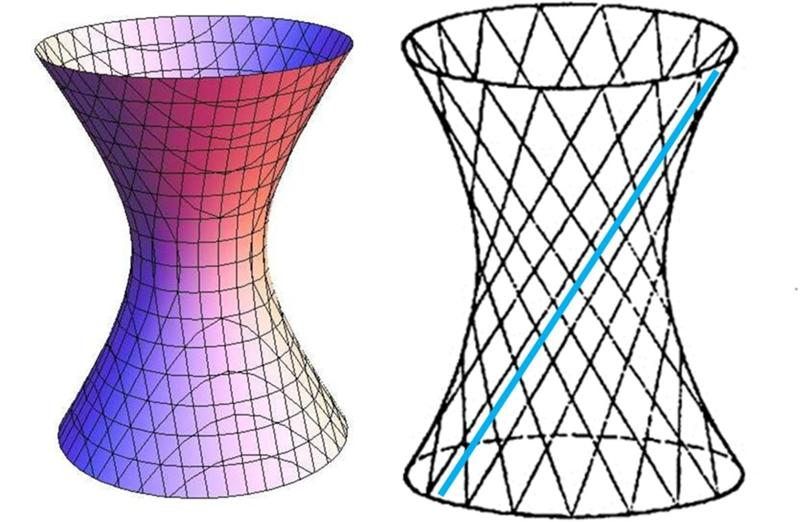
\includegraphics[width=0.5\linewidth]{гиперболоид.jpg}
% \end{center}
\indent Приведем к главным осям\footnote{Квадратичная форма в главных осях выглядит так: $Q=\lambda_1x_1^2+\ldots+\lambda_nx_n^2$, где $\lambda_1\ldots\lambda_n$ — собственные значения. Для приведения к главным осям находим собственные значения и векторы} квадратичную форму $2y^2-3z^2+4xz$. Составим ее матрицу
$$Q=\begin{pmatrix}
    0&0&2\\
    0&2&0\\
    2&0&-3
\end{pmatrix}$$
Ищем собственные значения\\[2mm]
$\begin{vmatrix}
    -\lambda&0&2\\
    0&2-\lambda&0\\
    2&0&-3-\lambda
\end{vmatrix}=0\Longrightarrow \lambda_1=-4, \lambda_2=1, \lambda_3=2$\\[2mm]
Так как у симметричной матрицы разные собственные значения, то собственные векторы ортогональны\\[2mm]
$\boxed{\text{Для }\lambda=2:}\begin{pmatrix}
    -2&0&2\\
    0&0&0\\
    2&0&-5
\end{pmatrix}\rightsquigarrow\begin{pmatrix}
    1&0&-1\\
    0&0&-3
\end{pmatrix}\rightsquigarrow\begin{pmatrix}
    1&0&-1\\
    0&0&1
\end{pmatrix}\rightsquigarrow\begin{pmatrix}
    1&0&0\\
    0&0&1
\end{pmatrix}\Longrightarrow v_1=\begin{pmatrix}
    0\\
    1\\
    0
\end{pmatrix}$\\[2mm]
$\boxed{\text{Для }\lambda=-4:}$ $v_2=\begin{pmatrix}
    -1\\
    0\\
    2
\end{pmatrix}\cdot\displaystyle\frac{1}{\sqrt{5}}$\\[2mm]
$\boxed{\text{Для }\lambda=1:}$ $v_3=\begin{pmatrix}
    2\\
    0\\
    1
\end{pmatrix}\cdot\displaystyle\frac{1}{\sqrt{5}}$\\[2mm]
Мы определили собственные вектора $(v_3, v_1, v_2)$, соответствующие собственным значениям $(1, 2, -4)$\\[2mm]
Тогда форма $Q$ будет такой:
$$Q=(x')^2+2(y')^2-4(z')^2$$
Матрица перехода $$C=\begin{pmatrix}
    \frac{2}{\sqrt{5}}&0&-\frac{1}{\sqrt{5}}\\[1mm]
    0&1&0\\[1mm]
    \frac{1}{\sqrt{5}}&0&\frac{2}{\sqrt{5}}
\end{pmatrix}$$
Добавим к форме линейную часть исходного уравнения и получим\footnote{$y'$ появился при умножении матрицы перехода на $(x',y',z')^T$}:
$$(x')^2+2(y')^2-4(z')^2-12y'+a=0$$
Теперь про параллельный перенос:

\begin{center}
    $(x')^2+2\left((y')^2-6y'+9\right)-18-4(z')^2+a=0$\\[2mm]
    $(x')^2+2(y'-3)^2-4(z')^2=18-a$
\end{center}
Сделаем замену $$\begin{cases}
    x'=x''\\
    (y'-3)=y''\\
    z'=z''
\end{cases}\Longleftrightarrow\begin{cases}
    x'=x''\\
    y'=y''+3\\
    z'=z''
\end{cases}$$
Получаем
\begin{equation}\label{eq:1}
    (x'')^2+2(y'')^2-4(z'')^2=18-a
\end{equation}
Рассмотрим случаи:
\begin{enumerate}
    \item Если $18-a>0$, то это точно однополосный гиперболоид, т.к. можно поделить уравнение \ref{eq:1} на $18-a$ и получить \href{https://cf.ppt-online.org/files/slide/e/EtDYxu4J1PBMHOnvFjdN9XrKephwIfS82yUlcm/slide-10.jpg}{каноническое уравнение гиперболоида}
    \item Если $18-a=0$, то мы получим конус
    \item Если $18-a<0$, то получим \href{https://cf.ppt-online.org/files1/slide/a/a8fSsCDgw0o64mQKNFPlhEWLUrO37zB9iGJTybIkt/slide-22.jpg}{двуполостный гиперболоид}
\end{enumerate}
Таким образом, выражение старых координат через новые:
$$\begin{aligned}
    \begin{pmatrix}
        x\\
        y\\
        z
    \end{pmatrix}&=C\begin{pmatrix}
        x'\\
        y'\\
        z'
    \end{pmatrix}\\
    &=C\left(\begin{pmatrix}
        x''\\
        y''\\
        z''
    \end{pmatrix}+\begin{pmatrix}
        0\\
        3\\
        0
    \end{pmatrix}\right)\\
    &=C\begin{pmatrix}
        x'\\
        y'\\
        z'
    \end{pmatrix}+\begin{pmatrix}
        0\\
        3\\
        0
    \end{pmatrix}
\end{aligned}$$

\newpage



\begin{tcolorbox}[colback=blue!20!white, colframe=black!100!black]
    \textbf{2021/2022. Вариант 1. Задача 4.} Приведите пример двух недиагонализуемых линейных операторов $\varphi, \psi$ в $\mathbb{R}^2$, для которых оператор $5\varphi-2\psi$ диагонализуем и отличен от нуля
\end{tcolorbox}
Оператор недиагонализуем, если его матрица недиагональна, а характеристический многочлен 
\begin{equation}\label{eq:2}
    (k-\lambda)^2+b>0,
\end{equation} то есть не имеет корней\\[2mm]
Пусть есть матрицы операторов $$5\varphi=\begin{pmatrix}
    a&b\\
    c&d
\end{pmatrix},\quad -2\psi=\begin{pmatrix}
    a'&b'\\
    c'&d'
\end{pmatrix}$$
Чтобы получить выражение \ref{eq:2} для матрицы $5\varphi$ расположим на главной диагонали одинаковые числа, например 1. Тогда мы получим часть $(k-\lambda)^2$\\[2mm]
На побочной диагонали разместим числа с противоположными знаками\\[2mm]
В матрице $-2\psi$ на главной диагонали расположим 0, а на побочной — числа, противоположные соответствующим числам в матрице $5\varphi$
\begin{equation*}
    5\varphi=\begin{pmatrix}
    1&-1\\
    1&1
\end{pmatrix},\quad -2\psi=\begin{pmatrix}
    0&1\\
    -1&0
\end{pmatrix}
\end{equation*}
Очевидно, что по отдельности каждая матрица не диагональна, а в сумме они дают диагональную матрицу\\[2mm]
Чтобы получить сами операторы $\varphi,\psi$ просто разделим матрицы на $5$ и $-2$ соответственно


\newpage


\begin{tcolorbox}[colback=blue!20!white, colframe=black!100!black]
    \textbf{2021/2022. Вариант 1. Задача 8.} Линейный оператор $\varphi:\mathbb{R}^4\rightarrow\mathbb{R}^4$ имеет в стандартном базисе матрицу 
    \begin{equation*}
    \begin{pmatrix}
        5&5&-1&-3\\
        0&3&0&0\\
        4&4&1&-6\\
        0&2&0&3
    \end{pmatrix}
    \end{equation*}
    Найдите базис пространства $\mathbb{R}^4$, в котором матрица оператора $\varphi$ имеет жорданову форму, и укажите эту жорданову форму
\end{tcolorbox}
\begin{equation*}
    \begin{vmatrix}
        5-\lambda&5&-1&-3\\
        0&3-\lambda&0&0\\
        4&4&1-\lambda&-6\\
        0&2&0&3-\lambda
    \end{vmatrix}=0\Longrightarrow \lambda=3
\end{equation*}
$\boxed{\text{Для }\lambda=3:}$ $\begin{pmatrix}
    2&5&-1&-3\\
    0&0&0&0\\
    4&4&-2&-6\\
    0&2&0&0
\end{pmatrix}\rightsquigarrow\begin{pmatrix}
    2&0&-1&-3\\
    0&0&0&0\\
    4&0&-2&-6\\
    0&2&0&0
\end{pmatrix}\Longrightarrow\rk{A}=2$\\[2mm]
$d_1=2$ — количество жардановых клеток, а также размерность соответствующего ядра\\[2mm]
$B=A-3E$\\[2mm]
$d_2=4-\rk{(B^2)}=4$\\[2mm]
$d_2-d_1=2\Longrightarrow$ количество жардановых клеток размером $\geqslant2$ равно двум\\[2mm]
Это означает, что жардановы клетки имеют размер $2\times2$\\[2mm]
Жорданова нормальная форма матрицы:
$$\left(
\begin{array}{cc|cc}
3 & 1 & 0 & 0 \\
 &  3 & 0 & 0 \\
\hline
0 & 0  & 3 & 1\\
0 & 0  &  & 3
\end{array}
\right)$$
$B=\begin{pmatrix}
    2&5&-1&-3\\
    0&0&0&0\\
    4&4&-2&-6\\
    0&2&0&0
\end{pmatrix}$\\[2mm]
Применим эту матрицу к базисным векторам
\begin{equation*}
    \underbrace{e_1}_{f_2}\xlongrightarrow{B}\underbrace{\begin{pmatrix}
        2\\
        0\\
        4\\
        0
    \end{pmatrix}}_{f_1}\xlongrightarrow{B}\begin{pmatrix}
        0\\
        0\\
        0\\
        0
    \end{pmatrix}
\end{equation*}
\begin{equation*}
    \underbrace{e_2}_{f_4}\xlongrightarrow{B}\underbrace{\begin{pmatrix}
        5\\
        0\\
        4\\
        2
    \end{pmatrix}}_{f_3}\xlongrightarrow{B}\begin{pmatrix}
        0\\
        0\\
        0\\
        0
    \end{pmatrix}
\end{equation*}
Проверим линейную независимость
\begin{equation*}
    \begin{pmatrix}
        e_1\\
        f_1\\
        f_3\\
        e_2
    \end{pmatrix}=\begin{pmatrix}
        1&0&0&0\\
        2&0&4&0\\
        5&0&4&2\\
        0&1&0&0
    \end{pmatrix}\rightsquigarrow\begin{pmatrix}
        0&0&0&0\\
        0&0&4&0\\
        0&0&4&2\\
        0&0&0&0
    \end{pmatrix}\text{не выражаются друг через друга} \Longrightarrow\text{линейно независимы}
\end{equation*}
Значит, $(f_1, f_2, f_3, f_4)$ — жорданов базис



\newpage

\begin{tcolorbox}[colback=blue!20!white, colframe=black!100!black]
    \textbf{2021/2022. Вариант 1. Задача 1.} Определите все значения, которые может принимать размерность суммы ядра и образа линейного оператора $\varphi:\mathbb{R}^4\rightarrow\mathbb{R}^4$ при условии, что в образе не содержится вектор $v=(1, 0, -1, 2)$
\end{tcolorbox}
$\dim{\ker{\varphi}}+\dim{\im{\varphi}}=4$\\[2mm]
\indent $\dim{(\ker{\varphi}+\im{\varphi})}=4-\dim{(\ker{\varphi}\cap\im{\varphi})}$\\[2mm]
\indent Пусть $\dim{(\ker{\varphi}\cap\im{\varphi})}=k$, тогда $k\leqslant2$\\[2mm]
\indent Проверим: если $k\geqslant3$, тогда 
$$\begin{aligned}
    \begin{cases}
    \dim{\ker{\varphi}}\geqslant3\\
    \dim{\im{\varphi}}\geqslant3
    \end{cases}\Longrightarrow\dim{(\ker{\varphi}+\im{\varphi})}\geqslant6,\text{ чего не может быть}
\end{aligned}$$
\indent Значит, возможные значения $k=0,1,2$\\[2mm]
\indent Распределим базисные векторы и $v$ так, чтобы $\dim{(\ker{\varphi}\cap\im{\varphi})}=0$\\[2mm]
\indent Так как $v\notin\im{\varphi}$, то $v\in\ker{\varphi}$ и 
$$\begin{aligned}
    v:&(1, 0, -1, 2)\longrightarrow(0, 0, 0, 0)
\end{aligned}$$
\indent Дополним $v$ векторами $e_1, e_2, e_3$ до базиса всего пространства\\[2mm]
\indent Сами вектора переведем в самих себя
$$\begin{aligned}
    e_1:&(1, 0, 0, 0)\longrightarrow(1, 0, 0, 0)\\
    e_2:&(0, 1, 0, 0)\longrightarrow(0, 1, 0, 0)\\
    e_3:&(0, 0, 1, 0)\longrightarrow(0, 0, 1, 0)\\
    v:&(1, 0, -1, 2)\longrightarrow(0, 0, 0, 0)
\end{aligned}$$
\indent Тогда, $\dim{(\ker{\varphi}\cap\im{\varphi})}=0$, так как $e_1, e_2, e_3$ линейно независимы\\[2mm]
\indent Последующие случаи рассматриваются аналогично

\newpage

\begin{tcolorbox}[colback=blue!20!white, colframe=black!100!black]
    \begin{center}
        \textbf{Ссылки}
    \end{center}
\end{tcolorbox}

\begin{enumerate}
    \item \href{https://disk.yandex.ru/i/cqWXCh6r0FtTuA}{Видео—разбор}
    \item \href{https://www.dropbox.com/sh/znsdw2ghc9lys05/AABlKcSZ-6sz4I7gBQfW63dva/LA_20-21_Stream2_Exam2.pdf?dl=0}{Экзамен 2020/2021}
    \item \href{https://drive.google.com/file/d/15N4-o5bWsfXrHJlkA_RpXX-7aX_Dkc6p/view?usp=sharing}{Экзамен 2021/2022}
\end{enumerate}




\end{document}
